\documentclass[10pt,a4paper]{article}

\usepackage[utf8]{inputenc}
\usepackage[T1]{fontenc}
\usepackage{lmodern}
\usepackage{microtype}
\usepackage[margin=0.48in,top=0.52in,bottom=0.48in,headheight=12pt,headsep=8pt,footskip=15pt]{geometry}
\usepackage{amsmath,amssymb,amsfonts}
\usepackage{booktabs}
\usepackage{array}
\usepackage{graphicx}
\usepackage{xcolor}
\usepackage{caption}
\usepackage{fancyhdr}
\usepackage[colorlinks=true,linkcolor=teal!70!black,urlcolor=teal!75!black,citecolor=teal!75!black]{hyperref}

\definecolor{headerteal}{HTML}{087F8C}
\definecolor{darkslate}{HTML}{17313B}

\captionsetup{font=footnotesize,labelfont={bf,color=darkslate},skip=3pt}

\makeatletter
\renewcommand\section{\@startsection {section}{1}{\z@}%
  {-7pt \@plus -2pt \@minus -1pt}%
  {3pt \@plus 1pt}%
  {\normalfont\large\bfseries\color{darkslate}}}
\renewcommand\subsection{\@startsection{subsection}{2}{\z@}%
  {-5pt \@plus -1pt \@minus -1pt}%
  {2pt \@plus 1pt}%
  {\normalfont\normalsize\bfseries\color{headerteal}}}
\makeatother

\pagestyle{fancy}
\fancyhf{}
\fancyhead[L]{\footnotesize\textcolor{darkslate}{\textbf{Chemical Engineering Thermodynamics Project Report:} \texttt{realgas-ml} v0.3.0}}
\fancyhead[R]{\footnotesize\textcolor{darkslate}{S.\ Gupta (2025CH11012) \& U.\ Jaipuria (2025CH11729)}}
\fancyfoot[C]{\footnotesize\textcolor{darkslate}{Page \thepage\ of 4}}
\renewcommand{\headrulewidth}{0.4pt}
\renewcommand{\footrulewidth}{0.4pt}

\setlength{\parindent}{0pt}
\setlength{\parskip}{2.2pt}
\AtBeginDocument{\fontsize{9.2}{11.0}\selectfont\setlength{\abovedisplayskip}{4pt}\setlength{\belowdisplayskip}{4pt}\setlength{\intextsep}{4pt}\setlength{\textfloatsep}{5pt}}
\renewcommand{\arraystretch}{0.96}

\begin{document}

\begin{center}
    {\LARGE\bfseries\color{darkslate} Dense-Data Local Quintic Radial-Basis-Function Surrogates for Peng--Robinson Real-Gas Thermodynamics (\texttt{realgas-ml} v0.3.0)}\\[5pt]
    {\normalsize \textbf{Satwik Gupta} (Roll No.\ \texttt{2025CH11012}) \quad and \quad \textbf{Udhav Jaipuria} (Roll No.\ \texttt{2025CH11729})}\\[2pt]
    {\footnotesize Department of Chemical Engineering $\cdot$ Chemical Engineering Thermodynamics Project $\cdot$ November 2026 $\cdot$ \href{https://github.com/satwikgupta122/realgas_ml}{GitHub Repository: \texttt{realgas\_ml}}}
\end{center}
\vspace{-4pt}
\noindent\textcolor{headerteal}{\rule{\textwidth}{0.8pt}}
\vspace{-8pt}

\section{Executive Summary and Thermodynamic Formulation}

The \href{https://github.com/satwikgupta122/realgas_ml}{\texttt{realgas-ml} (v0.3.0)} software package (\href{https://github.com/satwikgupta122/realgas_ml/blob/main/pyproject.toml}{\texttt{pyproject.toml}}, \href{https://github.com/satwikgupta122/realgas_ml/blob/main/README.md}{\texttt{README.md}}) implements a self-contained thermodynamic calculation engine and local kernel regression framework that predicts the pressure--volume--temperature ($PVT$), caloric, and phase-equilibrium departure properties of 15 pure supercritical fluids. Rather than relying on external runtime thermophysical libraries such as CoolProp or Cantera, the project synthesizes $65{,}536$ analytical states per fluid ($983{,}040$ states in total) directly from the classical \href{https://doi.org/10.1021/i160057a011}{Peng and Robinson (1976) two-constant cubic equation of state (PR76)} coupled with continuous \href{https://ntrs.nasa.gov/citations/19940013151}{NASA 7-coefficient ideal-gas heat-capacity polynomials}. Each fluid is represented by a four-output local quintic radial-basis-function (\texttt{LocalRBFRegressor}) surrogate trained over a normalized temperature and logarithmic-pressure grid.

In the analytical solver \href{https://github.com/satwikgupta122/realgas_ml/blob/main/realgas_ml/peng_robinson.py}{\texttt{realgas\_ml/peng\_robinson.py}}, pressure $P$ ($\mathrm{Pa}$) is expressed as a function of absolute temperature $T$ ($\mathrm{K}$) and molar volume $v$ ($\mathrm{m^3\,mol^{-1}}$) via the \href{https://doi.org/10.1021/i160057a011}{Peng--Robinson (1976) equation of state}:
\begin{equation}
P(T,v) = \frac{RT}{v - b} - \frac{a(T)}{v^2 + 2bv - b^2}, \qquad a(T) = a_c\left[1 + \kappa\left(1 - \sqrt{\frac{T}{T_c}}\right)\right]^2, \qquad b = 0.07780\,\frac{RT_c}{P_c}
\label{eq:pr76}
\end{equation}
where $R = 8.31446261815324\;\mathrm{J\,mol^{-1}\,K^{-1}}$ is the molar gas constant, $a_c = 0.45724\,R^2T_c^2/P_c$ denotes the critical attraction parameter, $T_c$ and $P_c$ represent the critical temperature and critical pressure, and $\kappa = 0.37464 + 1.54226\,\omega - 0.26992\,\omega^2$ is the original PR76 acentric polynomial in terms of Pitzer's acentric factor $\omega$. Differentiating $a(T)$ analytically with respect to temperature yields the first derivative required for caloric departure evaluations, $\frac{da}{dT} = -\frac{a_c\,\kappa\,g(T)}{T_c\sqrt{T/T_c}}$, where $g(T) = 1 + \kappa(1 - \sqrt{T/T_c})$. Defining the dimensionless attraction and covolume groups $A = \frac{a(T)P}{R^2T^2}$ and $B = \frac{bP}{RT}$, Equation~(\ref{eq:pr76}) is recast into the canonical cubic polynomial for the compressibility factor $Z = \frac{Pv}{RT}$:
\begin{equation}
Z^3 + (B - 1)Z^2 + (A - 3B^2 - 2B)Z + (-AB + B^2 + B^3) = 0
\label{eq:cubic_z}
\end{equation}
The function \texttt{cubic\_z(A, B)} in \href{https://github.com/satwikgupta122/realgas_ml/blob/main/realgas_ml/peng_robinson.py}{\texttt{peng\_robinson.py}} solves Equation~(\ref{eq:cubic_z}) at each state using companion-matrix eigenvalues (\texttt{numpy.roots}), filters physically admissible roots satisfying $|\operatorname{Im}(r)| < 10^{-9}$ and $\operatorname{Re}(r) > B$ (enforcing $v > b$), and selects the largest real root to isolate the single-phase gas branch.

To evaluate real-gas caloric and chemical-potential departures (\href{https://ejmaginn.github.io/CBE20260-notes/class34/fugacity-EOS.html}{Maginn, CBE 20260}), the solver defines the logarithmic factor $L$:
\begin{equation}
L = \ln\!\left[\frac{Z + (1 + \sqrt{2})B}{Z + (1 - \sqrt{2})B}\right] = \operatorname{log1p}\!\left[\frac{2\sqrt{2}\,B}{Z + (1 - \sqrt{2})B}\right]
\label{eq:log_factor}
\end{equation}
Evaluating $L$ via \texttt{np.log1p} in \href{https://github.com/satwikgupta122/realgas_ml/blob/main/realgas_ml/peng_robinson.py}{\texttt{peng\_robinson.py}} eliminates floating-point subtraction of nearly equal logarithms in the low-density limit ($P \to 1\;\mathrm{bar}$, $B \ll 1$, $Z \to 1$), preserving machine precision across all 15 fluids. The molar enthalpy departure $h_{\mathrm{dep}}$, molar entropy departure $s_{\mathrm{dep}}$, logarithmic fugacity coefficient $\ln\phi$, and fugacity $f$ are computed analytically as:
\begin{equation}
h_{\mathrm{dep}}(T,P) = RT(Z - 1) + \frac{T\frac{da}{dT} - a(T)}{2\sqrt{2}\,b}\,L, \qquad
s_{\mathrm{dep}}(T,P) = R\ln(Z - B) + \frac{\frac{da}{dT}}{2\sqrt{2}\,b}\,L
\label{eq:hs_dep}
\end{equation}
\begin{equation}
\ln\phi(T,P) = Z - 1 - \ln(Z - B) - \frac{A}{2\sqrt{2}\,B}\,L, \qquad f(T,P) = \phi(T,P)\,P
\label{eq:fugacity}
\end{equation}
Ideal-gas caloric contributions $h_{\mathrm{ig}}(T)$ and $s_{\mathrm{ig}}(T)$ are obtained in \texttt{ideal\_integrals(T, info)} by integrating the five heat-capacity coefficients $(a_0,\dots,a_4)$ of the \href{https://www.cantera.org/stable/reference/thermo/species-thermo.html}{NASA 7-coefficient polynomial} $C_p^\circ(T)/R = \sum_{k=0}^4 a_k T^k$ from the package reference state $T_{\mathrm{ref}} = 300.0\;\mathrm{K}$ and $P_{\mathrm{ref}} = 10^5\;\mathrm{Pa}$ ($1\;\mathrm{bar}$), where $h_{\mathrm{ig}}(T_{\mathrm{ref}}) = 0$ and $s_{\mathrm{ig}}(T_{\mathrm{ref}}, P_{\mathrm{ref}}) = 0$:
\begin{equation}
\tilde{h}(T) = R\!\left(a_0 T + \frac{a_1}{2}T^2 + \frac{a_2}{3}T^3 + \frac{a_3}{4}T^4 + \frac{a_4}{5}T^5\right), \quad
\tilde{s}(T) = R\!\left(a_0 \ln T + a_1 T + \frac{a_2}{2}T^2 + \frac{a_3}{3}T^3 + \frac{a_4}{4}T^4\right)
\label{eq:nasa7}
\end{equation}
The standard formation and third-law integration constants $(a_5, a_6)$ are intentionally omitted, and piecewise polynomial sub-intervals ($[200, 1000]\;\mathrm{K}$ and $[1000, 6000]\;\mathrm{K}$, or $[300, 1000, 5000]\;\mathrm{K}$ for $\mathrm{SO_2}$) are accumulated via clamped bounds (\texttt{np.clip}) to enforce exact $C^0$ continuity across the $1000\;\mathrm{K}$ midpoint junction (essential for $\mathrm{H_2O}$, whose domain extends to $1100.06\;\mathrm{K}$). Adding the real-gas departures yields total molar enthalpy $h(T,P) = h_{\mathrm{ig}}(T) + h_{\mathrm{dep}}(T,P)$ and total molar entropy $s(T,P) = s_{\mathrm{ig}}(T) - R\ln(P/P_{\mathrm{ref}}) + s_{\mathrm{dep}}(T,P)$. Because $h_{\mathrm{dep}}(300\;\mathrm{K}, 1\;\mathrm{bar}) \neq 0$, real-gas $h$ and $s$ are non-zero at the ideal-gas reference state.

\section{Fluid Domain Characterization and Thermophysical Provenance}

The dataset specification in \href{https://github.com/satwikgupta122/realgas_ml/blob/main/realgas_ml/data/metadata.json}{\texttt{realgas\_ml/data/metadata.json}} covers 15 pure fluids spanning monatomic noble gases ($\mathrm{He}$, $\mathrm{Ne}$, $\mathrm{Ar}$), homonuclear and heteronuclear diatomics ($\mathrm{H_2}$, $\mathrm{N_2}$, $\mathrm{O_2}$, $\mathrm{CO}$), linear and bent triatomics ($\mathrm{CO_2}$, $\mathrm{SO_2}$, $\mathrm{H_2O}$), polar associated hydrides ($\mathrm{NH_3}$), and the C$_1$--C$_4$ homologous $n$-alkane series ($\mathrm{CH_4}$, $\mathrm{C_2H_6}$, $\mathrm{C_3H_8}$, $n\text{-}\mathrm{C_4H_{10}}$). Static NASA7 polynomial arrays are sourced from \href{https://github.com/Cantera/cantera/blob/v3.2.0/data/nasa_gas.yaml}{Cantera 3.2.0 \texttt{nasa\_gas.yaml}} (\texttt{SHA-256: 4de6199d...8667e4db}, derived from \href{https://ntrs.nasa.gov/citations/19940013151}{NASA TM-4513}) under the BSD 3-Clause license preserved in \href{https://github.com/satwikgupta122/realgas_ml/blob/main/THIRD_PARTY_NOTICES.txt}{\texttt{THIRD\_PARTY\_NOTICES.txt}}. Critical constants ($T_c, P_c, \omega, M$) are transcribed from \href{https://github.com/Cantera/cantera/blob/v3.2.0/data/critical-properties.yaml}{Cantera 3.2.0 \texttt{critical-properties.yaml}} (referencing \href{https://doi.org/10.18434/T4D303}{Lemmon et al., 2022, NIST WebBook SRD 69}; Yaws, 2001; and Poling et al.) for nine species, and from static CoolProp fluid documentation tables for \href{https://coolprop.org/fluid_properties/fluids/Helium.html}{Helium}, \href{https://coolprop.org/fluid_properties/fluids/Argon.html}{Argon}, \href{https://coolprop.org/fluid_properties/fluids/Neon.html}{Neon}, \href{https://coolprop.org/fluid_properties/fluids/Ammonia.html}{Ammonia}, \href{https://coolprop.org/fluid_properties/fluids/SulfurDioxide.html}{SulfurDioxide}, and \href{https://coolprop.org/fluid_properties/fluids/Water.html}{Water}.

\begin{table}[ht!]
\centering
\caption{Thermophysical critical constants, operating domains ($P \in [1.0, 50.0]\;\mathrm{bar}$ for all fluids), reduced parameter bounds, and data provenance for all 15 pure fluids in \href{https://github.com/satwikgupta122/realgas_ml/blob/main/realgas_ml/data/metadata.json}{\texttt{metadata.json}}.}
\label{tab:fluids}
\footnotesize
\setlength{\tabcolsep}{3.8pt}
\resizebox{\textwidth}{!}{\begin{tabular}{llrrrrrrll}
\toprule
\textbf{Fluid Name} & \textbf{Species} & $M$ ($\mathrm{g\,mol^{-1}}$) & $T_c$ ($\mathrm{K}$) & $P_c$ ($\mathrm{bar}$) & $\omega$ (---) & $T_{\min}$ ($\mathrm{K}$) & $T_{\max}$ ($\mathrm{K}$) & $T_r = T/T_c$ Range & \textbf{Critical / NASA Provenance} \\
\midrule
Helium & $\mathrm{He}$ & 4.0026 & 5.1953 & 2.2832 & $-0.38354$ & 300.00 & 600.00 & $57.74\text{--}115.49$ & \href{https://coolprop.org/fluid_properties/fluids/Helium.html}{CoolProp He} / L10/90 \\
Hydrogen & $\mathrm{H_2}$ & 2.0159 & 32.9800 & 12.9300 & $-0.21700$ & 300.00 & 600.00 & $9.10\text{--}18.19$ & \href{https://github.com/Cantera/cantera/blob/v3.2.0/data/critical-properties.yaml}{Cantera (Poling)} / TPIS78 \\
Neon & $\mathrm{Ne}$ & 20.1790 & 44.4000 & 26.6163 & $-0.03549$ & 300.00 & 600.00 & $6.76\text{--}13.51$ & \href{https://coolprop.org/fluid_properties/fluids/Neon.html}{CoolProp Ne} / L10/90 \\
Nitrogen & $\mathrm{N_2}$ & 28.0135 & 126.2000 & 33.9000 & $0.03800$ & 300.00 & 600.00 & $2.38\text{--}4.75$ & \href{https://github.com/Cantera/cantera/blob/v3.2.0/data/critical-properties.yaml}{Cantera} (\href{https://doi.org/10.18434/T4D303}{NIST}) / TPIS78 \\
CarbonMonoxide & $\mathrm{CO}$ & 28.0101 & 133.4000 & 35.0000 & $0.06600$ & 300.00 & 499.00 & $2.25\text{--}3.74$ & \href{https://github.com/Cantera/cantera/blob/v3.2.0/data/critical-properties.yaml}{Cantera} (\href{https://doi.org/10.18434/T4D303}{NIST}) / TPIS79 \\
Argon & $\mathrm{Ar}$ & 39.9480 & 150.6870 & 48.6300 & $-0.00219$ & 300.00 & 600.00 & $1.99\text{--}3.98$ & \href{https://coolprop.org/fluid_properties/fluids/Argon.html}{CoolProp Ar} / L 6/88 \\
Oxygen & $\mathrm{O_2}$ & 31.9988 & 154.5800 & 50.4300 & $0.02200$ & 300.00 & 600.00 & $1.94\text{--}3.88$ & \href{https://github.com/Cantera/cantera/blob/v3.2.0/data/critical-properties.yaml}{Cantera} (\href{https://doi.org/10.18434/T4D303}{NIST}) / TPIS89 \\
Methane & $\mathrm{CH_4}$ & 16.0428 & 190.7000 & 46.3000 & $0.01100$ & 300.00 & 600.00 & $1.57\text{--}3.15$ & \href{https://github.com/Cantera/cantera/blob/v3.2.0/data/critical-properties.yaml}{Cantera} (\href{https://doi.org/10.18434/T4D303}{NIST}) / L 8/88 \\
CarbonDioxide & $\mathrm{CO_2}$ & 44.0098 & 304.2000 & 73.9000 & $0.22800$ & 334.62 & 600.00 & $1.10\text{--}1.97$ & \href{https://github.com/Cantera/cantera/blob/v3.2.0/data/critical-properties.yaml}{Cantera (Yaws)} / L 7/88 \\
Ethane & $\mathrm{C_2H_6}$ & 30.0690 & 305.4000 & 48.8000 & $0.09900$ & 335.94 & 600.00 & $1.10\text{--}1.96$ & \href{https://github.com/Cantera/cantera/blob/v3.2.0/data/critical-properties.yaml}{Cantera} (\href{https://doi.org/10.18434/T4D303}{NIST}) / L 8/88 \\
Propane & $\mathrm{C_3H_8}$ & 44.0956 & 369.7000 & 42.5000 & $0.15300$ & 406.88 & 628.81 & $1.10\text{--}1.70$ & \href{https://github.com/Cantera/cantera/blob/v3.2.0/data/critical-properties.yaml}{Cantera} (\href{https://doi.org/10.18434/T4D303}{NIST}) / L 6/90 \\
Ammonia & $\mathrm{NH_3}$ & 17.0305 & 405.5600 & 113.6339 & $0.25569$ & 446.12 & 689.45 & $1.10\text{--}1.70$ & \href{https://coolprop.org/fluid_properties/fluids/Ammonia.html}{CoolProp NH$_3$} / TPIS89 \\
$n$-Butane & $n\text{-}\mathrm{C_4H_{10}}$ & 58.1222 & 425.6000 & 37.6000 & $0.19900$ & 468.16 & 574.00 & $1.10\text{--}1.35$ & \href{https://github.com/Cantera/cantera/blob/v3.2.0/data/critical-properties.yaml}{Cantera} (\href{https://doi.org/10.18434/T4D303}{NIST}) / L 6/90 \\
SulfurDioxide & $\mathrm{SO_2}$ & 64.0638 & 430.6400 & 78.8658 & $0.25613$ & 473.70 & 524.00 & $1.10\text{--}1.22$ & \href{https://coolprop.org/fluid_properties/fluids/SulfurDioxide.html}{CoolProp SO$_2$} / J 6/61 \\
Water & $\mathrm{H_2O}$ & 18.0153 & 647.0960 & 220.6400 & $0.34429$ & 711.81 & 1100.06 & $1.10\text{--}1.70$ & \href{https://coolprop.org/fluid_properties/fluids/Water.html}{CoolProp H$_2$O} / L 8/89 \\
\bottomrule
\end{tabular}}
\end{table}

Table~\ref{tab:fluids} reveals the physical design of the state space. Every fluid shares the pressure domain $P \in [10^5,\, 5\times 10^6]\;\mathrm{Pa}$ ($1\text{--}50\;\mathrm{bar}$), while the minimum temperature satisfies $T_{\min} = \max(300.0\;\mathrm{K},\, 1.10\,T_c)$. Enforcing $T \ge 1.10\,T_c$ guarantees that every state lies strictly above the critical locus, preventing vapor--liquid phase splitting, Maxwell equal-area loops, and isothermal compressibility divergences $(\partial v/\partial P)_T \to -\infty$ at the critical point. Nevertheless, for high-$T_c$ hydrocarbons such as $n$-Butane ($P_c = 37.60\;\mathrm{bar}$), Propane ($P_c = 42.50\;\mathrm{bar}$), and Ethane ($P_c = 48.80\;\mathrm{bar}$), the upper pressure bound of $50\;\mathrm{bar}$ reaches reduced pressures $P_r = P_{\max}/P_c$ of $1.33$, $1.18$, and $1.02$, respectively, at reduced temperatures as low as $T_r = 1.10$. In this near-critical supercritical region, attractive intermolecular forces produce pronounced negative deviations from ideality ($Z \approx 0.65\text{--}0.85$) and steep gradients in $h_{\mathrm{dep}}$ and $\ln\phi$. Conversely, quantum and noble gases ($\mathrm{He}$, $\mathrm{H_2}$, $\mathrm{Ne}$) operate at $T_r \in [6.76, 115.49]$, where repulsive covolume interactions dominate ($Z > 1$) and thermodynamic surfaces are nearly planar.

\section{Surrogate Architecture, Coordinate Scaling, and Software Design}

The surrogate pipeline implemented across \href{https://github.com/satwikgupta122/realgas_ml/blob/main/train.py}{\texttt{train.py}}, \href{https://github.com/satwikgupta122/realgas_ml/blob/main/realgas_ml/regressor.py}{\texttt{realgas\_ml/regressor.py}}, and \href{https://github.com/satwikgupta122/realgas_ml/blob/main/realgas_ml/model.py}{\texttt{realgas\_ml/model.py}} addresses two numerical challenges inherent to real-gas property regression: multi-decade scale disparities across pressure and strict positivity constraints on compressibility and fugacity. Rather than fitting raw $(T, P)$ coordinates, \href{https://github.com/satwikgupta122/realgas_ml/blob/main/train.py}{\texttt{train.py}} and \href{https://github.com/satwikgupta122/realgas_ml/blob/main/realgas_ml/model.py}{\texttt{model.py}} map any physical state $(T, P) \in [T_{\min}, T_{\max}] \times [P_{\min}, P_{\max}]$ onto the unit square $\mathbf{x} = (x_1, x_2) \in [0, 1]^2$ via linear temperature normalization and logarithmic pressure scaling:
\begin{equation}
x_1(T) = \frac{T - T_{\min}}{T_{\max} - T_{\min}} \in [0, 1], \qquad
x_2(P) = \frac{\ln(P / P_{\min})}{\ln(P_{\max} / P_{\min})} \in [0, 1]
\label{eq:scaling}
\end{equation}
Logarithmic pressure scaling serves a dual mathematical purpose. First, because the ideal-gas entropy contains the exact term $-R\ln(P/P_{\mathrm{ref}})$, mapping $\ln P \mapsto x_2$ transforms this logarithmic singularity into an affine linear function of $x_2$ that is reproduced with zero error by the polynomial trend of the kernel interpolator. Second, uniform sampling in $x_2$ concentrates grid nodes geometrically toward lower pressures ($1\text{--}10\;\mathrm{bar}$) while maintaining balanced resolution across the 50-fold pressure ratio. The target vector is parameterized as $\mathbf{y} = [\ln Z,\; h,\; s,\; \ln\phi]^\top \in \mathbb{R}^4$. During inference in \href{https://github.com/satwikgupta122/realgas_ml/blob/main/realgas_ml/model.py}{\texttt{GasModel.predict}}, the predicted log-targets $\hat{y}_1$ and $\hat{y}_4$ are exponentiated ($Z = \exp(\hat{y}_1)$ and $\phi = \exp(\hat{y}_4)$), guaranteeing $Z > 0$ and $\phi > 0$ everywhere and reconstructing derived intensive and extensive properties for $n$ moles via exact algebraic definitions:
\begin{equation}
v = \frac{ZRT}{P}, \quad V = nv, \quad \rho = \frac{M}{v}, \quad H = n\hat{y}_2, \quad S = n\hat{y}_3, \quad f = \phi P
\label{eq:reconstruction}
\end{equation}
Crucially, as verified in \href{https://github.com/satwikgupta122/realgas_ml/blob/main/tests/test_properties.py}{\texttt{tests/test\_properties.py}} and \href{https://github.com/satwikgupta122/realgas_ml/blob/main/tests/test_app.py}{\texttt{tests/test\_app.py}}, fugacity $f$ is an intensive state variable and remains invariant with respect to molar amount $n$, whereas extensive volume $V$, enthalpy $H$, and entropy $S$ scale linearly with $n$.

In \href{https://github.com/satwikgupta122/realgas_ml/blob/main/realgas_ml/regressor.py}{\texttt{realgas\_ml/regressor.py}}, \texttt{LocalRBFRegressor} wraps SciPy's \texttt{RBFInterpolator} within a scikit-learn \texttt{BaseEstimator} and \texttt{RegressorMixin} interface. The four target columns are first standardized to zero mean and unit variance using \texttt{StandardScaler}. For any query state $\mathbf{x} \in [0, 1]^2$, the interpolator identifies the $k = 48$ nearest training nodes $\{\mathbf{x}_{i_1},\dots,\mathbf{x}_{i_k}\}$ in Euclidean norm and forms a local quintic radial-basis-function expansion augmented by a quadratic polynomial of degree $m = 2$ with zero smoothing ($\lambda = 0$, exact interpolation):
\begin{equation}
\tilde{\mathbf{y}}(\mathbf{x}) = \sum_{j=1}^{48} \mathbf{w}_j\,\varphi\!\left(\|\mathbf{x} - \mathbf{x}_{i_j}\|_2\right) + \sum_{\alpha_1 + \alpha_2 \le 2} \mathbf{c}_{\alpha_1,\alpha_2}\,x_1^{\alpha_1} x_2^{\alpha_2}, \qquad \varphi(r) = -r^5
\label{eq:rbf}
\end{equation}
where the weights $\mathbf{w}_j \in \mathbb{R}^4$ and polynomial coefficients $\mathbf{c}_{\alpha_1,\alpha_2} \in \mathbb{R}^4$ satisfy the $48$ interpolation constraints $\tilde{\mathbf{y}}(\mathbf{x}_{i_j}) = \mathbf{y}_{\mathrm{std}}(\mathbf{x}_{i_j})$ subject to $6$ discrete orthogonality conditions $\sum_{j=1}^{48} \mathbf{w}_j\,x_{i_j,1}^{\alpha_1} x_{i_j,2}^{\alpha_2} = \mathbf{0}$ for $\alpha_1 + \alpha_2 \le 2$. Whereas global RBF interpolation on $N = 65{,}536$ nodes would require factoring a dense $65{,}536 \times 65{,}536$ matrix ($\sim 34\;\mathrm{GB}$ in double precision and $\mathcal{O}(N^3) \approx 2.8\times 10^{14}$ operations), the $k=48$ local neighborhood reduces evaluation to a $k$-d tree query followed by solving a $54 \times 54$ linear system per query point. Each serialized model (\texttt{realgas\_ml/data/<Gas>.joblib}, compressed at level 3) occupies only $2.63\text{--}2.66\;\mathrm{MB}$ on disk.

For inverse $TV$ state specifications—where temperature $T$ and molar volume $v$ are known and pressure $P$ must be recovered—\texttt{GasModel.pressure(T, v)} in \href{https://github.com/satwikgupta122/realgas_ml/blob/main/realgas_ml/model.py}{\texttt{model.py}} defines the residual function $g(P) = \hat{v}(T, P) - v$, verifies opposite signs at the pressure domain brackets $g(P_{\min})\cdot g(P_{\max}) \le 0$, and executes Brent's root-finding algorithm (\texttt{scipy.optimize.brentq}) over $[10^5, 5\times 10^6]\;\mathrm{Pa}$. Because $(\partial v/\partial P)_T < 0$ for all stable single-phase gas states, $g(P)$ is strictly monotonic and Brent's method converges to machine precision ($\text{relative error} < 10^{-8}$ in \href{https://github.com/satwikgupta122/realgas_ml/blob/main/tests/test_properties.py}{\texttt{test\_properties.py}}). The package exposes four user interfaces: the Python API (\href{https://github.com/satwikgupta122/realgas_ml/blob/main/example.py}{\texttt{example.py}}), the command-line entry point \texttt{realgas-ml} (\href{https://github.com/satwikgupta122/realgas_ml/blob/main/realgas_ml/cli.py}{\texttt{realgas\_ml/cli.py}}), a bulk NPZ-to-CSV dataset exporter (\href{https://github.com/satwikgupta122/realgas_ml/blob/main/export_data.py}{\texttt{export\_data.py}}), and an interactive Streamlit web laboratory (\href{https://github.com/satwikgupta122/realgas_ml/blob/main/app.py}{\texttt{app.py}}, styled via \href{https://github.com/satwikgupta122/realgas_ml/blob/main/.streamlit/config.toml}{\texttt{.streamlit/config.toml}} and launched on Windows via \href{https://github.com/satwikgupta122/realgas_ml/blob/main/run_app.bat}{\texttt{run\_app.bat}}) supporting both $(T,P)$ and inverse $(T,v)$ modes, unit conversions ($\mathrm{K}$/$^\circ\mathrm{C}$, $\mathrm{bar}$/$\mathrm{kPa}$/$\mathrm{MPa}$/$\mathrm{Pa}$), 80-point geometric-pressure trend curves, and side-by-side PR residual tables.

\section{Empirical Accuracy, Convergence Scaling, and Thermodynamic Consistency}

The training protocol in \href{https://github.com/satwikgupta122/realgas_ml/blob/main/train.py}{\texttt{train.py}} employs a deterministic random generator (\texttt{np.random.default\_rng(20261016 + index)}) to partition the evaluation sets independently for each fluid: (i) a full $256 \times 256 = 65{,}536$ Cartesian training grid on $[0, 1]^2$; (ii) $512$ uniformly distributed interior validation points used exclusively to record multi-grid learning curves at $N \in \{32^2, 64^2, 128^2, 256^2\}$; (iii) $2{,}048$ uniformly distributed held-out interior test points; and (iv) $256$ held-out domain-boundary test points ($64$ random points along each of the four edges $x_1 \in \{0,1\}$ and $x_2 \in \{0,1\}$). Relative accuracy for positive-definite properties ($v$ and $f$) is quantified via Mean Absolute Percentage Error ($\mathrm{MAPE}$) and Maximum Absolute Percentage Error ($\mathrm{Max\;APE}$), derived directly from logarithmic residuals as $100\,|\exp(\hat{y} - y) - 1|$, while caloric accuracy for $h$ and $s$ (which cross zero near $300\;\mathrm{K}$ and $1\;\mathrm{bar}$) is measured via Mean Absolute Error ($\mathrm{MAE}$) and Maximum Absolute Error ($\mathrm{Max\;AE}$).

\begin{table}[ht!]
\centering
\caption{Held-out interior test ($N=2{,}048$) and domain-boundary test ($N=256$) surrogate errors against direct Peng--Robinson calculations for all 15 gases trained on the $256 \times 256$ ($65{,}536$-state) grid (extracted from \href{https://github.com/satwikgupta122/realgas_ml/tree/main/realgas_ml/data}{\texttt{realgas\_ml/data/*\_metrics.json}}).}
\label{tab:test_metrics}
\scriptsize
\setlength{\tabcolsep}{2.7pt}
\resizebox{\textwidth}{!}{\begin{tabular}{lrrrrrrrrrrrr}
\toprule
& \multicolumn{6}{c}{\textbf{Held-Out Interior Test Split ($N = 2{,}048$ Random States)}} & \multicolumn{6}{c}{\textbf{Held-Out Domain-Boundary Split ($N = 256$ Edge States)}} \\
\cmidrule(lr){2-7} \cmidrule(lr){8-13}
\textbf{Fluid (Metrics File)} & \textbf{$v$ MAPE} & \textbf{$v$ Max} & \textbf{$f$ MAPE} & \textbf{$f$ Max} & \textbf{$h$ MAE} & \textbf{$s$ MAE} & \textbf{$v$ MAPE} & \textbf{$v$ Max} & \textbf{$f$ MAPE} & \textbf{$f$ Max} & \textbf{$h$ Max AE} & \textbf{$s$ Max AE} \\
& \textbf{(\%)} & \textbf{APE (\%)} & \textbf{(\%)} & \textbf{APE (\%)} & \textbf{($\mathrm{J/mol}$)} & \textbf{($\mathrm{J/mol\,K}$)} & \textbf{(\%)} & \textbf{APE (\%)} & \textbf{(\%)} & \textbf{APE (\%)} & \textbf{($\mathrm{J/mol}$)} & \textbf{($\mathrm{J/mol\,K}$)} \\
\midrule
\href{https://github.com/satwikgupta122/realgas_ml/blob/main/realgas_ml/data/Helium_metrics.json}{Helium} & $3.46\text{e-}10$ & $4.94\text{e-}08$ & $2.80\text{e-}10$ & $3.90\text{e-}08$ & $1.02\text{e-}08$ & $2.55\text{e-}10$ & $1.23\text{e-}09$ & $1.38\text{e-}07$ & $9.38\text{e-}10$ & $9.68\text{e-}08$ & $2.19\text{e-}06$ & $1.22\text{e-}08$ \\
\href{https://github.com/satwikgupta122/realgas_ml/blob/main/realgas_ml/data/Neon_metrics.json}{Neon} & $5.49\text{e-}10$ & $7.84\text{e-}08$ & $5.66\text{e-}10$ & $8.28\text{e-}08$ & $1.98\text{e-}08$ & $3.14\text{e-}10$ & $5.25\text{e-}10$ & $2.59\text{e-}08$ & $5.46\text{e-}10$ & $2.56\text{e-}08$ & $7.37\text{e-}07$ & $1.73\text{e-}08$ \\
\href{https://github.com/satwikgupta122/realgas_ml/blob/main/realgas_ml/data/Hydrogen_metrics.json}{Hydrogen} & $6.47\text{e-}10$ & $7.74\text{e-}08$ & $6.10\text{e-}10$ & $7.26\text{e-}08$ & $3.23\text{e-}08$ & $3.32\text{e-}10$ & $8.94\text{e-}10$ & $6.60\text{e-}08$ & $7.94\text{e-}10$ & $4.95\text{e-}08$ & $2.44\text{e-}06$ & $2.82\text{e-}09$ \\
\href{https://github.com/satwikgupta122/realgas_ml/blob/main/realgas_ml/data/Water_metrics.json}{Water} & $9.96\text{e-}10$ & $8.60\text{e-}08$ & $9.53\text{e-}10$ & $7.32\text{e-}08$ & $4.53\text{e-}07$ & $4.37\text{e-}10$ & $1.47\text{e-}09$ & $3.34\text{e-}08$ & $1.14\text{e-}09$ & $2.36\text{e-}08$ & $6.54\text{e-}06$ & $6.53\text{e-}09$ \\
\href{https://github.com/satwikgupta122/realgas_ml/blob/main/realgas_ml/data/Nitrogen_metrics.json}{Nitrogen} & $1.16\text{e-}09$ & $3.12\text{e-}07$ & $1.06\text{e-}09$ & $2.46\text{e-}07$ & $4.16\text{e-}08$ & $4.22\text{e-}10$ & $1.84\text{e-}09$ & $5.90\text{e-}08$ & $1.83\text{e-}09$ & $5.43\text{e-}08$ & $2.09\text{e-}06$ & $2.23\text{e-}08$ \\
\href{https://github.com/satwikgupta122/realgas_ml/blob/main/realgas_ml/data/Oxygen_metrics.json}{Oxygen} & $1.30\text{e-}09$ & $1.90\text{e-}07$ & $1.10\text{e-}09$ & $1.20\text{e-}07$ & $6.17\text{e-}08$ & $4.57\text{e-}10$ & $2.20\text{e-}09$ & $9.14\text{e-}08$ & $2.09\text{e-}09$ & $7.17\text{e-}08$ & $1.77\text{e-}06$ & $1.78\text{e-}08$ \\
\href{https://github.com/satwikgupta122/realgas_ml/blob/main/realgas_ml/data/CarbonMonoxide_metrics.json}{CarbonMonoxide} & $1.37\text{e-}09$ & $2.81\text{e-}07$ & $1.11\text{e-}09$ & $1.72\text{e-}07$ & $4.30\text{e-}08$ & $1.78\text{e-}10$ & $2.07\text{e-}09$ & $1.98\text{e-}07$ & $1.54\text{e-}09$ & $1.05\text{e-}07$ & $1.95\text{e-}05$ & $6.15\text{e-}08$ \\
\href{https://github.com/satwikgupta122/realgas_ml/blob/main/realgas_ml/data/Argon_metrics.json}{Argon} & $1.39\text{e-}09$ & $2.72\text{e-}07$ & $1.19\text{e-}09$ & $1.78\text{e-}07$ & $6.19\text{e-}08$ & $3.25\text{e-}10$ & $1.87\text{e-}09$ & $3.31\text{e-}08$ & $1.81\text{e-}09$ & $3.18\text{e-}08$ & $8.65\text{e-}07$ & $5.36\text{e-}09$ \\
\href{https://github.com/satwikgupta122/realgas_ml/blob/main/realgas_ml/data/Methane_metrics.json}{Methane} & $1.85\text{e-}09$ & $1.60\text{e-}07$ & $1.45\text{e-}09$ & $8.28\text{e-}08$ & $1.16\text{e-}07$ & $5.04\text{e-}10$ & $1.06\text{e-}08$ & $1.37\text{e-}06$ & $7.71\text{e-}09$ & $8.10\text{e-}07$ & $3.61\text{e-}05$ & $2.00\text{e-}07$ \\
\href{https://github.com/satwikgupta122/realgas_ml/blob/main/realgas_ml/data/Ammonia_metrics.json}{Ammonia} & $2.27\text{e-}09$ & $2.14\text{e-}07$ & $2.09\text{e-}09$ & $1.87\text{e-}07$ & $4.53\text{e-}07$ & $6.38\text{e-}10$ & $5.90\text{e-}09$ & $5.11\text{e-}07$ & $3.24\text{e-}09$ & $2.50\text{e-}07$ & $4.70\text{e-}05$ & $9.10\text{e-}08$ \\
\href{https://github.com/satwikgupta122/realgas_ml/blob/main/realgas_ml/data/CarbonDioxide_metrics.json}{CarbonDioxide} & $4.78\text{e-}09$ & $9.96\text{e-}07$ & $2.71\text{e-}09$ & $4.80\text{e-}07$ & $3.78\text{e-}07$ & $7.16\text{e-}10$ & $2.47\text{e-}08$ & $2.84\text{e-}06$ & $9.46\text{e-}09$ & $7.60\text{e-}07$ & $8.98\text{e-}05$ & $3.59\text{e-}07$ \\
\href{https://github.com/satwikgupta122/realgas_ml/blob/main/realgas_ml/data/SulfurDioxide_metrics.json}{SulfurDioxide} & $1.07\text{e-}08$ & $1.98\text{e-}06$ & $5.74\text{e-}09$ & $7.47\text{e-}07$ & $1.43\text{e-}06$ & $2.40\text{e-}09$ & $1.09\text{e-}08$ & $4.29\text{e-}07$ & $5.34\text{e-}09$ & $1.62\text{e-}07$ & $4.74\text{e-}05$ & $8.64\text{e-}08$ \\
\href{https://github.com/satwikgupta122/realgas_ml/blob/main/realgas_ml/data/Ethane_metrics.json}{Ethane} & $1.73\text{e-}08$ & $7.53\text{e-}06$ & $5.38\text{e-}09$ & $1.06\text{e-}06$ & $8.64\text{e-}07$ & $2.17\text{e-}09$ & $5.28\text{e-}08$ & $2.25\text{e-}06$ & $1.39\text{e-}08$ & $4.26\text{e-}07$ & $1.75\text{e-}04$ & $4.74\text{e-}07$ \\
\href{https://github.com/satwikgupta122/realgas_ml/blob/main/realgas_ml/data/Propane_metrics.json}{Propane} & $1.85\text{e-}08$ & $5.63\text{e-}06$ & $4.65\text{e-}09$ & $4.77\text{e-}07$ & $1.09\text{e-}06$ & $2.23\text{e-}09$ & $4.66\text{e-}08$ & $8.53\text{e-}07$ & $1.09\text{e-}08$ & $1.53\text{e-}07$ & $6.82\text{e-}05$ & $1.62\text{e-}07$ \\
\href{https://github.com/satwikgupta122/realgas_ml/blob/main/realgas_ml/data/n-Butane_metrics.json}{$n$-Butane} & $4.08\text{e-}08$ & $9.48\text{e-}06$ & $6.99\text{e-}09$ & $3.41\text{e-}07$ & $2.16\text{e-}06$ & $3.89\text{e-}09$ & $8.28\text{e-}08$ & $\mathbf{1.04\text{e-}05}$ & $1.12\text{e-}08$ & $\mathbf{1.50\text{e-}06}$ & $\mathbf{4.10\text{e-}04}$ & $\mathbf{8.24\text{e-}07}$ \\
\midrule
\textbf{Global Worst Case} & $\mathbf{4.08\text{e-}08}$ & $\mathbf{9.48\text{e-}06}$ & $\mathbf{6.99\text{e-}09}$ & $\mathbf{1.06\text{e-}06}$ & $\mathbf{2.16\text{e-}06}$ & $\mathbf{3.89\text{e-}09}$ & $\mathbf{8.28\text{e-}08}$ & $\mathbf{1.04\text{e-}05}$ & $\mathbf{1.39\text{e-}08}$ & $\mathbf{1.50\text{e-}06}$ & $\mathbf{4.10\text{e-}04}$ & $\mathbf{8.24\text{e-}07}$ \\
\bottomrule
\end{tabular}}
\end{table}

Table~\ref{tab:test_metrics} and Figure~\ref{fig:errors} demonstrate that across all 15 fluids and both held-out interior and boundary test sets, the maximum relative error on molar volume is $1.0365 \times 10^{-5}\%$ ($n$-Butane boundary), the maximum relative error on fugacity is $1.4985 \times 10^{-6}\%$ ($n$-Butane boundary), the maximum absolute error on molar enthalpy is $4.0967 \times 10^{-4}\;\mathrm{J\,mol^{-1}}$ ($n$-Butane boundary), and the maximum absolute error on molar entropy is $8.2417 \times 10^{-7}\;\mathrm{J\,mol^{-1}\,K^{-1}}$ ($n$-Butane boundary). These worst-case figures lie three to four orders of magnitude below the automated regression gates enforced in \href{https://github.com/satwikgupta122/realgas_ml/blob/main/tests/test_properties.py}{\texttt{tests/test\_properties.py}} ($\mathrm{Max\;APE} < 0.01\%$ for $v$ and $f$, $\mathrm{Max\;AE} < 0.5\;\mathrm{J\,mol^{-1}}$ for $h$, and $\mathrm{Max\;AE} < 0.005\;\mathrm{J\,mol^{-1}\,K^{-1}}$ for $s$).

\begin{figure}[ht!]
\centering
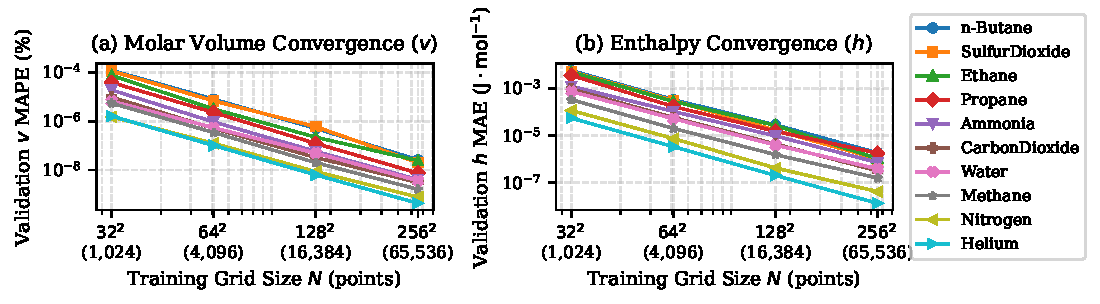
\includegraphics[width=0.94\textwidth]{fig_learning_curves.pdf}
\vspace{-2pt}
\caption{Validation learning curves ($N_{\mathrm{val}} = 512$) across grid resolutions $N \in \{32^2, 64^2, 128^2, 256^2\}$ for (a) molar volume MAPE and (b) molar enthalpy MAE, illustrating uniform $\sim \mathcal{O}(\Delta x^{3.8\text{--}4.1})$ algebraic error decay with mesh refinement.}
\label{fig:learning}
\end{figure}

\begin{figure}[ht!]
\centering
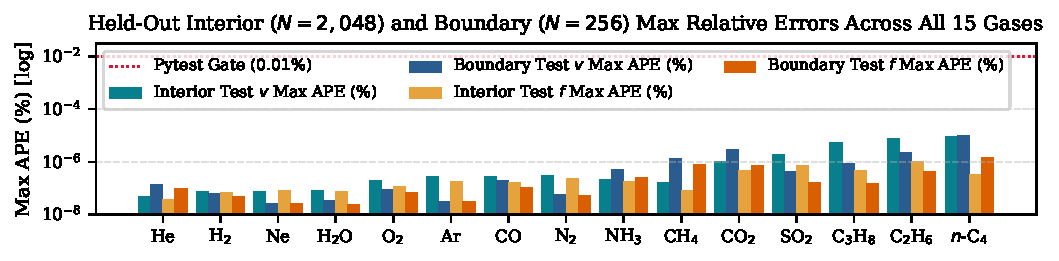
\includegraphics[width=0.94\textwidth]{fig_test_boundary_errors.pdf}
\vspace{-2pt}
\caption{Comparison of held-out interior test ($N=2{,}048$) and domain-boundary ($N=256$) maximum relative errors on molar volume $v$ and fugacity $f$ across all 15 fluids at $N=65{,}536$, benchmarked against the $0.01\%$ acceptance gate in \href{https://github.com/satwikgupta122/realgas_ml/blob/main/tests/test_properties.py}{\texttt{test\_properties.py}}.}
\label{fig:errors}
\end{figure}

A physical hierarchy governs the error variation across fluids in Table~\ref{tab:test_metrics}. Because local quintic RBF interpolation with quadratic polynomial precision ($m=2$) annihilates all Taylor series terms up to second order, the local truncation error at grid spacing $\Delta x = 1/(M_{\mathrm{side}}-1)$ is proportional to high-order mixed partial derivatives $\partial^{\alpha_1+\alpha_2} \mathbf{y} / \partial x_1^{\alpha_1} \partial x_2^{\alpha_2}$ ($|\boldsymbol{\alpha}| \ge 3$). For Helium ($T_r \ge 57.7$), Neon ($T_r \ge 6.76$), and Hydrogen ($T_r \ge 9.10$), the compressibility surface $Z(T,P)$ is nearly flat and close to unity, yielding interior molar volume MAPEs between $3.46\times 10^{-10}\%$ and $6.47\times 10^{-10}\%$. Notably, Water exhibits similarly low interior volume MAPE ($9.96\times 10^{-10}\%$) despite its high acentricity ($\omega = 0.3443$) and polarity because its maximum pressure of $50\;\mathrm{bar}$ represents a small reduced pressure $P_{\max}/P_c = 50 / 220.64 = 0.2266$ at $T \ge 711.81\;\mathrm{K}$, keeping supercritical steam in a weakly non-ideal regime throughout the domain. In contrast, $n$-Butane, Propane, and Ethane experience $P_{\max}/P_c \in [1.02, 1.33]$ near $T_{\min} = 1.10\,T_c$, where the supercritical inflection of $Z(T,P)$ across the Widom extension of the coexistence curve maximizes third- and fourth-order derivatives. Even for these strongly non-ideal alkanes, boundary errors exceed interior errors by at most a factor of $2\text{--}5\times$, confirming that the 48-neighbor asymmetric stencil and degree-2 polynomial reproduction suppress Runge-phenomenon boundary oscillations.

\begin{table}[ht!]
\centering
\caption{Validation learning-curve progression ($N_{\mathrm{val}} = 512$) across the four training grid densities $N \in \{1{,}024,\; 4{,}096,\; 16{,}384,\; 65{,}536\}$ for all 15 gases, showing average step reduction factor $\overline{\rho}_{4\times} = \frac{1}{3}\sum_{k=1}^3 (\mathrm{Error}_{N_k}/\mathrm{Error}_{N_{k+1}})$ and effective spatial convergence rate $p_{\mathrm{eff}} = \log_2(\overline{\rho}_{4\times})$.}
\label{tab:learning_curve}
\scriptsize
\setlength{\tabcolsep}{3.1pt}
\resizebox{\textwidth}{!}{\begin{tabular}{lrrrrrrrrrr}
\toprule
& \multicolumn{5}{c}{\textbf{Validation Molar Volume $\mathrm{MAPE}$ (\%) vs.\ Grid Size $N$}} & \multicolumn{5}{c}{\textbf{Validation Molar Enthalpy $\mathrm{MAE}$ ($\mathrm{J\,mol^{-1}}$) vs.\ Grid Size $N$}} \\
\cmidrule(lr){2-6} \cmidrule(lr){7-11}
\textbf{Fluid} & $N=1{,}024$ & $N=4{,}096$ & $N=16{,}384$ & $N=65{,}536$ & $p_{\mathrm{eff}}(v)$ & $N=1{,}024$ & $N=4{,}096$ & $N=16{,}384$ & $N=65{,}536$ & $p_{\mathrm{eff}}(h)$ \\
\midrule
Helium & $1.62\text{e-}06$ & $1.01\text{e-}07$ & $6.28\text{e-}09$ & $4.33\text{e-}10$ & $3.95$ & $5.38\text{e-}05$ & $3.28\text{e-}06$ & $1.96\text{e-}07$ & $1.29\text{e-}08$ & $4.01$ \\
Water & $1.50\text{e-}06$ & $1.23\text{e-}07$ & $8.55\text{e-}09$ & $7.80\text{e-}10$ & $3.64$ & $7.28\text{e-}04$ & $5.10\text{e-}05$ & $3.83\text{e-}06$ & $3.77\text{e-}07$ & $3.64$ \\
Neon & $1.82\text{e-}06$ & $1.07\text{e-}07$ & $8.70\text{e-}09$ & $5.99\text{e-}10$ & $3.86$ & $7.12\text{e-}05$ & $4.35\text{e-}06$ & $3.56\text{e-}07$ & $2.51\text{e-}08$ & $3.82$ \\
Hydrogen & $2.79\text{e-}06$ & $1.83\text{e-}07$ & $1.35\text{e-}08$ & $1.28\text{e-}09$ & $3.70$ & $1.50\text{e-}04$ & $9.14\text{e-}06$ & $6.08\text{e-}07$ & $4.87\text{e-}08$ & $3.86$ \\
Oxygen & $3.62\text{e-}06$ & $2.60\text{e-}07$ & $2.34\text{e-}08$ & $1.88\text{e-}09$ & $3.64$ & $1.17\text{e-}04$ & $6.68\text{e-}06$ & $5.19\text{e-}07$ & $5.63\text{e-}08$ & $3.68$ \\
Argon & $4.85\text{e-}06$ & $2.65\text{e-}07$ & $1.75\text{e-}08$ & $1.73\text{e-}09$ & $3.82$ & $1.18\text{e-}04$ & $9.52\text{e-}06$ & $6.12\text{e-}07$ & $6.33\text{e-}08$ & $3.62$ \\
CarbonMonoxide & $5.41\text{e-}06$ & $3.83\text{e-}07$ & $2.47\text{e-}08$ & $2.07\text{e-}09$ & $3.78$ & $1.13\text{e-}04$ & $7.06\text{e-}06$ & $5.34\text{e-}07$ & $5.56\text{e-}08$ & $3.66$ \\
Nitrogen & $5.45\text{e-}06$ & $3.44\text{e-}07$ & $2.00\text{e-}08$ & $1.61\text{e-}09$ & $3.91$ & $1.14\text{e-}04$ & $7.28\text{e-}06$ & $4.08\text{e-}07$ & $4.06\text{e-}08$ & $3.82$ \\
Ammonia & $6.60\text{e-}06$ & $5.38\text{e-}07$ & $4.87\text{e-}08$ & $3.65\text{e-}09$ & $3.61$ & $1.21\text{e-}03$ & $1.03\text{e-}04$ & $9.37\text{e-}06$ & $6.98\text{e-}07$ & $3.59$ \\
Methane & $9.70\text{e-}06$ & $5.04\text{e-}07$ & $3.24\text{e-}08$ & $3.07\text{e-}09$ & $3.87$ & $3.29\text{e-}04$ & $1.97\text{e-}05$ & $1.51\text{e-}06$ & $1.53\text{e-}07$ & $3.69$ \\
CarbonDioxide & $1.90\text{e-}05$ & $9.29\text{e-}07$ & $5.76\text{e-}08$ & $4.04\text{e-}09$ & $4.06$ & $9.23\text{e-}04$ & $5.69\text{e-}05$ & $4.27\text{e-}06$ & $3.08\text{e-}07$ & $3.85$ \\
SulfurDioxide & $3.85\text{e-}05$ & $2.26\text{e-}06$ & $1.22\text{e-}07$ & $7.47\text{e-}09$ & $4.11$ & $5.14\text{e-}03$ & $2.99\text{e-}04$ & $1.64\text{e-}05$ & $1.00\text{e-}06$ & $4.11$ \\
Propane & $7.52\text{e-}05$ & $3.16\text{e-}06$ & $2.20\text{e-}07$ & $2.42\text{e-}08$ & $3.86$ & $3.54\text{e-}03$ & $1.67\text{e-}04$ & $1.49\text{e-}05$ & $1.74\text{e-}06$ & $3.66$ \\
Ethane & $1.13\text{e-}04$ & $6.76\text{e-}06$ & $5.94\text{e-}07$ & $2.00\text{e-}08$ & $4.16$ & $4.88\text{e-}03$ & $2.75\text{e-}04$ & $2.63\text{e-}05$ & $1.02\text{e-}06$ & $4.08$ \\
$n$-Butane & $1.21\text{e-}04$ & $7.91\text{e-}06$ & $5.06\text{e-}07$ & $2.60\text{e-}08$ & $4.06$ & $5.76\text{e-}03$ & $3.27\text{e-}04$ & $2.77\text{e-}05$ & $1.79\text{e-}06$ & $3.88$ \\
\bottomrule
\end{tabular}}
\end{table}

Table~\ref{tab:learning_curve} and Figure~\ref{fig:learning} quantify the validation convergence across four successive dyadic grid refinements ($M_{\mathrm{side}} \in \{32, 64, 128, 256\}$, where each $4\times$ increase in $N$ halves the mesh spacing $\Delta x$). Across all 15 fluids, halving $\Delta x$ reduces validation $\mathrm{MAPE}$ and $\mathrm{MAE}$ by a factor of $12.2\times$ to $17.9\times$, yielding an effective empirical convergence order $p_{\mathrm{eff}} \in [3.59, 4.16]$. Consequently, refining from $32 \times 32$ ($1{,}024$ points) to $256 \times 256$ ($65{,}536$ points) reduces surrogate errors by more than three orders of magnitude ($\sim 2{,}000\times$ to $5{,}600\times$) without encountering conditioning breakdown.

To verify physical self-consistency of the underlying dataset, \href{https://github.com/satwikgupta122/realgas_ml/blob/main/tests/test_properties.py}{\texttt{tests/test\_properties.py}} executes 47 automated tests across all 15 fluids at $T_{\mathrm{mid}} = (T_{\min} + T_{\max})/2$ and $P = 2.0\;\mathrm{MPa}$ using central finite differences ($\Delta T = 0.01\;\mathrm{K}$, $\Delta P = 100.0\;\mathrm{Pa}$), confirming five fundamental thermodynamic identities to within relative tolerances of $10^{-10}$ to $2\times 10^{-5}$:
\begin{equation}
g_{\mathrm{dep}} = h_{\mathrm{dep}} - T s_{\mathrm{dep}} = RT\ln\phi, \; \left(\frac{\partial h}{\partial P}\right)_T = v - T\left(\frac{\partial v}{\partial T}\right)_P, \; \left(\frac{\partial s}{\partial P}\right)_T = -\left(\frac{\partial v}{\partial T}\right)_P, \; \left(\frac{\partial \ln f}{\partial P}\right)_T = \frac{v}{RT}, \; \left(\frac{\partial h}{\partial T}\right)_P = T\left(\frac{\partial s}{\partial T}\right)_P
\label{eq:maxwell}
\end{equation}

\section{Conclusions, Limitations, and Engineering Implications}

The \href{https://github.com/satwikgupta122/realgas_ml}{\texttt{realgas-ml} v0.3.0} architecture demonstrates that pairing logarithmic pressure normalization and logarithmic target transforms ($\ln Z, \ln\phi$) with local quintic RBF interpolation ($k=48, m=2$) reproduces analytical Peng--Robinson and NASA7 thermodynamics across 15 pure fluids to 8--10 significant digits ($\mathrm{Max\;APE} \le 1.04\times 10^{-5}\%$). By eliminating iterative cubic root finding during forward evaluations and bounding inverse $P(T,v)$ queries within Brent's method, the package provides fast, dependency-free property lookups suitable for process simulation teaching laboratories and offline engineering workflows. Two fundamental engineering caveats documented in \href{https://github.com/satwikgupta122/realgas_ml/blob/main/README.md}{\texttt{README.md}} and \href{https://github.com/satwikgupta122/realgas_ml/blob/main/realgas_ml/model.py}{\texttt{model.py}} warrant emphasis. First, because the four targets $[\ln Z, h, s, \ln\phi]$ are interpolated as independent scalar fields, the surrogate's analytical partial derivatives satisfy Equation~(\ref{eq:maxwell}) only up to the $\sim 10^{-8}$ interpolation residual rather than identically; differential sensitivity solvers requiring exact Jacobian symmetry should invoke \texttt{peng\_robinson.properties} directly or fit a single scalar fundamental potential (such as molar Helmholtz energy $a(T,v)$) and differentiate it analytically. Second, the reported errors quantify numerical fidelity to the PR76 equation of state, not physical accuracy against experimental measurements; PR76 exhibits known structural deviations for strongly polar hydrogen-bonding fluids ($\mathrm{H_2O}, \mathrm{NH_3}$) and quantum fluids ($\mathrm{He}, \mathrm{H_2}$), where multi-parameter Helmholtz equations of state remain necessary for custody-transfer precision.

\section*{References and Repository Provenance}
\vspace{-2pt}
{\footnotesize
\begin{enumerate}\setlength{\itemsep}{1pt}\setlength{\parskip}{0pt}
    \item Peng, D.-Y., \& Robinson, D.\ B.\ (1976). A New Two-Constant Equation of State. \textit{Industrial \& Engineering Chemistry Fundamentals}, 15(1), 59--64. \href{https://doi.org/10.1021/i160057a011}{https://doi.org/10.1021/i160057a011}
    \item McBride, B.\ J., Gordon, S., \& Reno, M.\ A.\ (1993). \textit{Coefficients for Calculating Thermodynamic and Transport Properties of Individual Species}. NASA Technical Memorandum 4513. \href{https://ntrs.nasa.gov/citations/19940013151}{https://ntrs.nasa.gov/citations/19940013151}
    \item Cantera Developers (2025). \textit{Cantera 3.2.0 Species Thermodynamic Polynomials} (\href{https://www.cantera.org/stable/reference/thermo/species-thermo.html}{Species Thermo Reference}), \href{https://github.com/Cantera/cantera/blob/v3.2.0/data/nasa_gas.yaml}{\texttt{nasa\_gas.yaml}}, and \href{https://github.com/Cantera/cantera/blob/v3.2.0/data/critical-properties.yaml}{\texttt{critical-properties.yaml}}. License notices retained in \href{https://github.com/satwikgupta122/realgas_ml/blob/main/THIRD_PARTY_NOTICES.txt}{\texttt{THIRD\_PARTY\_NOTICES.txt}}.
    \item Lemmon, E.\ W., Bell, I.\ H., Huber, M.\ L., \& McLinden, M.\ O.\ (2022). Thermophysical Properties of Fluid Systems. In \textit{NIST Chemistry WebBook, NIST Standard Reference Database Number 69}. \href{https://doi.org/10.18434/T4D303}{https://doi.org/10.18434/T4D303}
    \item Bell, I.\ H., et al.\ (CoolProp Fluid Documentation): Static critical parameters for \href{https://coolprop.org/fluid_properties/fluids/Helium.html}{Helium}, \href{https://coolprop.org/fluid_properties/fluids/Neon.html}{Neon}, \href{https://coolprop.org/fluid_properties/fluids/Argon.html}{Argon}, \href{https://coolprop.org/fluid_properties/fluids/Ammonia.html}{Ammonia}, \href{https://coolprop.org/fluid_properties/fluids/SulfurDioxide.html}{SulfurDioxide}, and \href{https://coolprop.org/fluid_properties/fluids/Water.html}{Water}.
    \item Maginn, E.\ J.\ \textit{CBE 20260 Lecture Notes: Fugacity from Equations of State}. University of Notre Dame. \href{https://ejmaginn.github.io/CBE20260-notes/class34/fugacity-EOS.html}{CBE20260 Fugacity-EOS Notes}
    \item Project Repository (\href{https://github.com/satwikgupta122/realgas_ml}{\texttt{realgas\_ml}}): \href{https://github.com/satwikgupta122/realgas_ml/blob/main/README.md}{\texttt{README.md}}, \href{https://github.com/satwikgupta122/realgas_ml/blob/main/pyproject.toml}{\texttt{pyproject.toml}}, \href{https://github.com/satwikgupta122/realgas_ml/blob/main/realgas_ml/peng_robinson.py}{\texttt{peng\_robinson.py}}, \href{https://github.com/satwikgupta122/realgas_ml/blob/main/realgas_ml/regressor.py}{\texttt{regressor.py}}, \href{https://github.com/satwikgupta122/realgas_ml/blob/main/realgas_ml/model.py}{\texttt{model.py}}, \href{https://github.com/satwikgupta122/realgas_ml/blob/main/train.py}{\texttt{train.py}}, \href{https://github.com/satwikgupta122/realgas_ml/blob/main/app.py}{\texttt{app.py}}, \href{https://github.com/satwikgupta122/realgas_ml/blob/main/realgas_ml/cli.py}{\texttt{cli.py}}, \href{https://github.com/satwikgupta122/realgas_ml/blob/main/export_data.py}{\texttt{export\_data.py}}, \href{https://github.com/satwikgupta122/realgas_ml/blob/main/realgas_ml/data/metadata.json}{\texttt{metadata.json}}, \href{https://github.com/satwikgupta122/realgas_ml/blob/main/tests/test_properties.py}{\texttt{test\_properties.py}}, and \href{https://github.com/satwikgupta122/realgas_ml/blob/main/tests/test_app.py}{\texttt{test\_app.py}}.
\end{enumerate}
}

\end{document}
